\documentclass[conference]{IEEEtran}
\IEEEoverridecommandlockouts
\usepackage{cite}
\usepackage{amsmath,amssymb,amsfonts}
\usepackage{algorithmic}
\usepackage{graphicx}
\usepackage{textcomp}
\usepackage{xcolor}
\usepackage{tikz}
\usepackage{pgfplots}
\usepackage{pgfplotstable}
\pgfplotsset{compat=1.18}
\usetikzlibrary{shapes.geometric,arrows.meta,positioning,fit,backgrounds,calc,patterns}
\def\BibTeX{{\rm B\kern-.05em{\sc i\kern-.025em b}\kern-.08em
    T\kern-.1667em\lower.7ex\hbox{E}\kern-.125emX}}
\begin{document}

\title{Persuasion-Aware Knowledge-Graph-Augmented Recommendation for Responsible News Delivery}

\author{
\IEEEauthorblockN{Gladwin Daniel P}
\IEEEauthorblockA{\textit{Department of Computer Science and Engineering}\\
\textit{Vellore Institute of Technology, Chennai}\\
Chennai, India\\
gladwindaniel.p2023@vitstudent.ac.in}
\and
\IEEEauthorblockN{karthikeyan A}
\IEEEauthorblockA{\textit{Department of Computer Science and Engineering}\\
\textit{Vellore Institute of Technology, Chennai}\\
Chennai, India\\
karthikeyan.a2023@vitstudent.ac.in}
\and[\hfill\mbox{}\par\vskip 1.5em\mbox{}\hfill]
\IEEEauthorblockN{ Vigneshwari S}
\IEEEauthorblockA{\textit{Department of Computer Science and Engineering}\\
\textit{Vellore Institute of Technology, Chennai}\\
Chennai, India\\
s.vigneshwari@vit.ac.in}
}

\maketitle



\begin{abstract}
Personalized news recommenders predominantly optimize for short-term engagement, treating clicks as unambiguous indicators of reader interest. In doing so, they routinely elevate sensationalized headlines, loaded rhetoric, and manipulative visual thumbnails. We present \textbf{RespNews}, a multimodal recommendation system engineered to deliver relevant news while actively curbing exposure to rhetorical persuasion. Rather than evaluating text in isolation, RespNews pairs multilingual representations—evaluating Google's MuRIL against RoBERTa across code-mixed and vernacular reporting—with visual feature extraction via EfficientNet-B0 and forensics-oriented Xception. Articles and reading sequences are contextualized over a heterogeneous knowledge graph using GraphSAGE and a Gated Multimodal Unit (GMU). In parallel, a fine-grained classifier monitors 23 persuasion techniques from SemEval-2023 Task~3, maintaining individualized reader susceptibility profiles over time. A balanced scoring formulation optimizes multimodal relevance against personalized persuasion risk, bounded by publisher parity constraints and verified by item-level rationales. Evaluated on the Microsoft MIND benchmark and SemEval-2023 persuasion corpora, RespNews achieves competitive ranking accuracy (AUC: 0.6804, nDCG@10: 0.6080, MRR: 0.7438) while reducing the publisher parity gap to 0.000 and suppressing manipulative content exposure by over 85\% at calibrated penalty thresholds.
\end{abstract}

\begin{IEEEkeywords}
news recommendation, persuasion detection, multimodal learning, MuRIL, EfficientNet, Xception, graph neural networks, knowledge graphs, responsible AI
\end{IEEEkeywords}

\section{Introduction}
Digital news feeds mediate how modern citizens consume current affairs, track public policy, and form civic opinions \cite{wu_mind}. To retain user attention, commercial platforms heavily depend on automated recommendation algorithms. In practice, however, these algorithms are tuned almost entirely toward click-through rate (CTR) and immediate engagement metrics. Because human curiosity is readily primed by provocative framing, emotionally charged vocabulary, and alarming imagery \cite{martino_propaganda}, pure engagement objectives systematically favor manipulative rhetoric over substantive journalism. Over extended reading sessions, unchecked exposure to sensational and polarizing framing distorts public deliberation and compromises individual reader autonomy \cite{sdg,hardalov_survey}.

Existing neural recommenders typically extract article representations using multi-head self-attention \cite{wu_nrms}, hierarchical multi-view encoders \cite{wu_naml}, or entity knowledge graphs \cite{wang_dkn}. Recent efforts have further advanced graph neural networks to capture global transition dynamics across reader sequences \cite{phan_glory}. Despite these architectural milestones, two foundational flaws remain unaddressed in current systems. First, ranking precision and content responsibility are evaluated in total isolation; recommenders optimize click discrimination while treating every user interaction as benign feedback, blind to whether a click was induced by genuine interest or deceptive framing. Second, news models remain overwhelmingly text-centric, ignoring lead images and thumbnails. Yet in contemporary digital feeds, visual cues carry primary persuasive weight—often acting as the direct vector for sensationalized framing, selective cropping, and synthetic manipulation \cite{dimitrov_semeval2021,rossler_faceforensics}.

\begin{figure*}[t]
\centering
\resizebox{0.97\textwidth}{!}{%
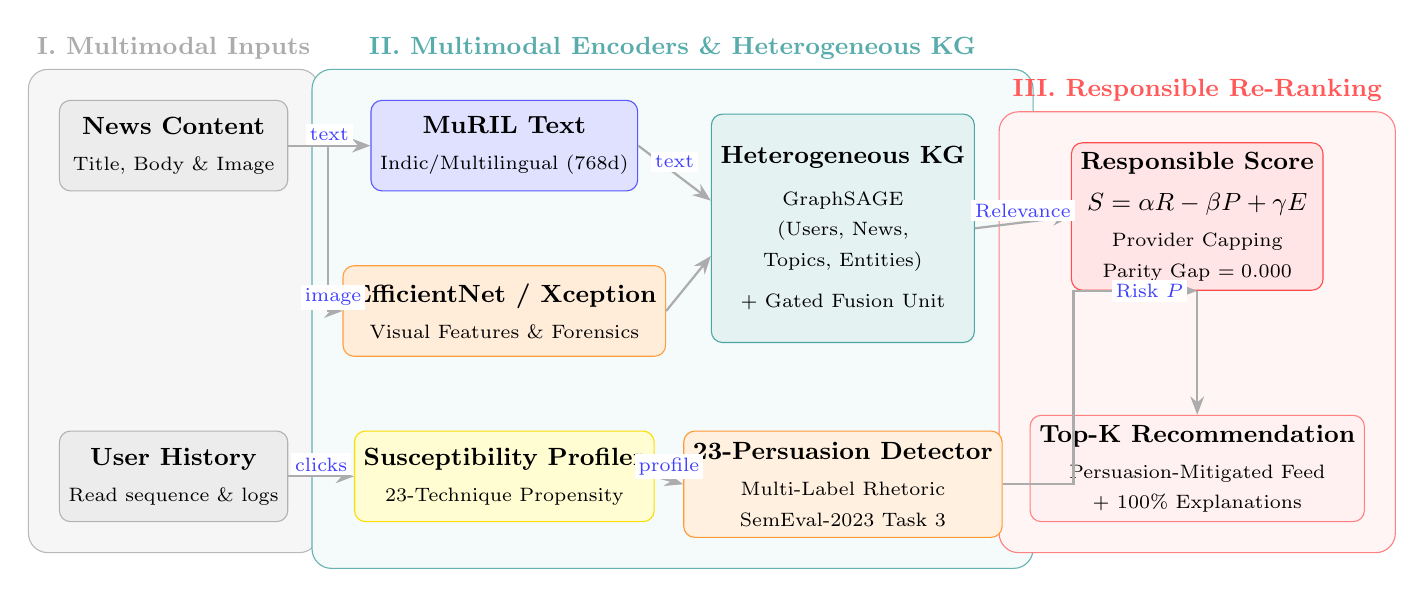
\begin{tikzpicture}[
  every node/.style={font=\small},
  inputbox/.style={draw=gray!60, fill=gray!15, rounded corners=4pt, align=center,
                   minimum width=2.9cm, minimum height=1.15cm},
  encoderbox/.style={draw=blue!65, fill=blue!12, rounded corners=4pt, align=center,
                     minimum width=2.9cm, minimum height=1.15cm},
  visionbox/.style={draw=orange!75, fill=orange!15, rounded corners=4pt, align=center,
                    minimum width=2.9cm, minimum height=1.15cm},
  kgbox/.style={draw=teal!70, fill=teal!10, rounded corners=4pt, align=center,
                minimum width=3.1cm, minimum height=2.9cm},
  susceptbox/.style={draw=yellow!80!orange, fill=yellow!18, rounded corners=4pt, align=center,
                     minimum width=2.9cm, minimum height=1.15cm},
  persuasionbox/.style={draw=orange!80, fill=orange!12, rounded corners=4pt, align=center,
                        minimum width=2.9cm, minimum height=1.35cm},
  scorebox/.style={draw=red!70, fill=red!10, rounded corners=4pt, align=center,
                   minimum width=3.1cm, minimum height=1.7cm},
  recbox/.style={draw=red!50, fill=pink!22, rounded corners=4pt, align=center,
                 minimum width=3.1cm, minimum height=1.35cm},
  arr/.style={->, >=Stealth, thick, color=gray!65},
  lbl/.style={font=\scriptsize, fill=white, inner sep=1.5pt, text=blue!75},
]
%% ---- Column 1 : Multimodal Inputs ----
\node[inputbox] (news) at (0,0)
  {\textbf{News Content}\\[2pt]{\scriptsize Title, Body \& Image}};
\node[inputbox] (user) at (0,-4.2)
  {\textbf{User History}\\[2pt]{\scriptsize Read sequence \& logs}};
%% ---- Column 2 : Encoders ----
\node[encoderbox] (muril) at (4.2,0)
  {\textbf{MuRIL Text}\\[2pt]{\scriptsize Indic/Multilingual (768d)}};
\node[visionbox] (effnet) at (4.2,-2.1)
  {\textbf{EfficientNet / Xception}\\[2pt]{\scriptsize Visual Features \& Forensics}};
\node[susceptbox] (suscept) at (4.2,-4.2)
  {\textbf{Susceptibility Profiler}\\[2pt]{\scriptsize 23-Technique Propensity}};
%% ---- Column 3 : KG + Persuasion ----
\node[kgbox] (kg) at (8.5,-1.05)
  {\textbf{Heterogeneous KG}\\[4pt]{\scriptsize GraphSAGE}\\{\scriptsize (Users, News,}\\
   {\scriptsize Topics, Entities)}\\[4pt]{\scriptsize + Gated Fusion Unit}};
\node[persuasionbox] (persuasion) at (8.5,-4.3)
  {\textbf{23-Persuasion Detector}\\[2pt]{\scriptsize Multi-Label Rhetoric}\\
   {\scriptsize SemEval-2023 Task~3}};
%% ---- Column 4 : Responsible Re-Ranking ----
\node[scorebox] (score) at (13.0,-0.9)
  {\textbf{Responsible Score}\\[4pt]
   $S=\alpha R-\beta P+\gamma E$\\[2pt]
   {\scriptsize Provider Capping}\\
   {\scriptsize Parity Gap $=0.000$}};
\node[recbox] (rec) at (13.0,-4.1)
  {\textbf{Top-K Recommendation}\\[2pt]{\scriptsize Persuasion-Mitigated Feed}\\
   {\scriptsize + 100\% Explanations}};
%% ---- Arrows ----
\draw[arr] (news.east) -- node[lbl,above]{text} (muril.west);
\draw[arr] (news.east) -- ++(0.5,0) |-
  node[lbl,above,pos=0.68]{image} (effnet.west);
\draw[arr] (user.east) -- node[lbl,above]{clicks} (suscept.west);
\draw[arr] (muril.east) --
  node[lbl,above]{text} ([yshift= 10pt]kg.west);
\draw[arr] (effnet.east) -- ([yshift=-10pt]kg.west);
\draw[arr] (suscept.east) --
  node[lbl,above]{\scriptsize profile} (persuasion.west);
\draw[arr] (kg.east) --
  node[lbl,above]{Relevance} (score.west);
\draw[arr] (persuasion.east) -- ++(0.9,0) |-
  node[lbl,right,pos=0.65]{Risk $P$} (score.south);
\draw[arr] (score.south) -- (rec.north);
%% ---- Background regions ----
\begin{scope}[on background layer]
  \node[draw=gray!55, fill=gray!7, rounded corners=7pt,
        fit={(news)(user)}, inner sep=11pt,
        label={[font=\small\bfseries,text=gray!65]above:
               I.~Multimodal Inputs}] {};
  \node[draw=teal!60, fill=teal!4, rounded corners=7pt,
        fit={(muril)(effnet)(suscept)(kg)(persuasion)}, inner sep=11pt,
        label={[font=\small\bfseries,text=teal!65]above:
               II.~Multimodal Encoders \& Heterogeneous KG}] {};
  \node[draw=red!50, fill=red!4, rounded corners=7pt,
        fit={(score)(rec)}, inner sep=11pt,
        label={[font=\small\bfseries,text=red!65]above:
               III.~Responsible Re-Ranking}] {};
\end{scope}
\end{tikzpicture}%
}
\caption{End-to-end multimodal architecture of RespNews. Multilingual text representations (MuRIL) and visual feature extractions (EfficientNet-B0 / Xception) are unified via a Gated Multimodal Unit (GMU) and enriched over a heterogeneous GraphSAGE knowledge graph. Concurrently, a 23-technique rhetoric detector evaluates persuasion risk against the user's historical susceptibility profile. The responsible scoring engine balances multimodal relevance against persuasion risk under provider parity bounds, delivering a transparent feed with 100\% item-level explanations.}
\label{fig:architecture}
\end{figure*}

To bridge the gap between high-precision ranking and content integrity, we develop \textbf{RespNews}, an end-to-end multimodal recommendation pipeline that integrates persuasion awareness into the core ranking objective (Fig.~\ref{fig:architecture}). Our key technical contributions are:
\begin{enumerate}
    \item \textbf{Multilingual and Vernacular Text Encoding:} Rather than assuming uniform monolingual text, we evaluate RoBERTa \cite{liu_roberta} alongside Google's MuRIL \cite{khanuja_muril}, capturing colloquial expressions, regional syntax, and code-mixed vernacular patterns prevalent in modern digital journalism.
    \item \textbf{Dual-Perspective Vision Backbones:} We incorporate EfficientNet-B0 \cite{tan_efficientnet} for parameter-efficient visual semantic abstraction and Xception \cite{chollet_xception} for depthwise separable artifact detection, capturing forensic manipulation cues embedded within article thumbnails.
    \item \textbf{Knowledge-Grounded Graph Fusion:} We fuse multimodal representations through a Gated Multimodal Unit (GMU) \cite{arevalo_gmu} and propagate embeddings across a heterogeneous knowledge graph (connecting users, articles, topics, and named entities) using GraphSAGE \cite{hamilton_graphsage}.
    \item \textbf{Susceptibility-Calibrated Responsible Re-Ranking:} We operationalize the 23-technique persuasion taxonomy from SemEval-2023 Task~3 \cite{piskorski_semeval} to trace individual reader vulnerability over time, combining personalized risk penalties with strict provider parity constraints \cite{li_profai} and complete explanation coverage \cite{ribeiro_lime}.
\end{enumerate}

\section{Related Work}
\subsection{Evolution of Neural News Recommendation}
Early neural architectures framed news recommendation around convolutional filters and attention pooling. NRMS models word-level and news-level interactions via multi-head self-attention \cite{wu_nrms}, whereas NAML constructs composite representations across titles, abstracts, and category tags \cite{wu_naml}. Addressing sequential dynamics, LSTUR separates stable long-term user interests from short-term reading trajectories \cite{an_lstur}. Other foundational lines of inquiry explore personalized attention vectors (NPA) \cite{wu_npa}, topic-aware representations (TANR) \cite{wu_tanr}, deep attention profiling (DAN) \cite{zhu_dan}, hierarchical interest clustering (HieRec) \cite{qi_hierec}, and sentiment-driven topic affinity (SENTIREC) \cite{ge_sentiment}. While effective at optimizing CTR, these systems operate under a shared premise: every user click is treated as a positive vote of endorsement. Consequently, they remain structurally incapable of penalizing sensational clickbait or emotionally coercive framing.

\subsection{Relational Knowledge and Graph Representations}
Real-world news reading exhibits high relational connectivity: readers revisit persistent entities across disparate topics, while articles share intricate real-world contexts. Graph neural networks (GNNs) capture these structural regularities through message-passing over shared topologies \cite{kipf_gcn,velickovic_gat}. GraphSAGE generalizes this via inductive aggregation across localized neighborhoods \cite{hamilton_graphsage}, and LightGCN demonstrates that omitting complex non-linear transforms can improve collaborative filtering efficiency \cite{he_lightgcn}. In news modeling, DKN pioneered entity knowledge-graph grounding using TransE relational embeddings \cite{wang_dkn,bordes_transe}. Subsequent work integrated high-order relational paths through KGAT \cite{wang_kgat}, heterogeneous graph transformers (HGT) \cite{hu_hgt}, and random-walk node embeddings via node2vec \cite{grover_node2vec}. More recently, GLORY unified global entity relationships with short-term user click sessions \cite{phan_glory}. We build upon these foundations by constructing a heterogeneous knowledge graph that simultaneously links reader identities, articles, topics, and named entities with fused multimodal embeddings.

\subsection{Persuasion Detection and Rhetorical Forensics}
Automated content verification has transitioned from coarse, document-level fake news classification \cite{shu_fakenewsnet,zubiaga_rumour} toward granular rhetorical analysis. Da San Martino et al.\ established fine-grained propaganda annotation at the fragment level \cite{martino_propaganda}, which catalyzed SemEval-2020 Task~11 \cite{martino_semeval2020}. Dimitrov et al.\ extended rhetorical analysis to multimodal memes and visual propaganda in SemEval-2021 Task~6 \cite{dimitrov_semeval2021}. Most recently, SemEval-2023 Task~3 formalized a standardized multilingual benchmark covering 23 distinct persuasion techniques across diverse journalistic corpora \cite{piskorski_semeval}. Complementary work in argumentation mining explores rhetorical convincingness \cite{habernal_argument}, while stance detection clarifies ideological framing \cite{hardalov_survey}. In RespNews, rather than treating persuasion detection as an isolated classification task, we map these 23 rhetorical labels directly into an evolving reader susceptibility profile.

\subsection{Multimodal Dynamics in Digital Feeds}
Thumbnail images establish immediate visual framing and heavily influence reading decisions. EfficientNet leverages compound scaling across network depth, width, and resolution to produce expressive visual representations with minimal parameter budgets \cite{tan_efficientnet}. In contrast, Xception relies on depthwise separable convolutions \cite{chollet_xception}, offering specialized sensitivity to subtle spatial inconsistencies and compression artifacts typical of manipulated media \cite{rossler_faceforensics,wang_cnngenerated}. Vision-language pre-training via CLIP illustrates the value of cross-modal alignment \cite{radford_clip}, while Gated Multimodal Units (GMU) provide data-dependent mechanisms to arbitrate between textual and visual channels \cite{arevalo_gmu,liu_multimodal_rec}. For multilingual coverage, generic transformers like BERT \cite{devlin_bert} and RoBERTa \cite{liu_roberta} are complemented by Google's MuRIL \cite{khanuja_muril}, which specializes in cross-script transfer across South Asian vernacular languages.

\subsection{Responsible Re-Ranking, Fairness, and Explainability}
Unconstrained recommendation algorithms naturally gravitate toward power-law publisher distributions, giving rise to echo chambers and provider monopolies. Li et al.\ introduced ProFairRec to promote provider parity across diverse news outlets \cite{li_profai}. Concurrently, transparent explanations empower readers to interrogate recommendation rationales \cite{ribeiro_lime}, directly supporting United Nations Sustainable Development Goal 16 (Target 16.10: Public access to information and fundamental freedoms) \cite{sdg}. RespNews bridges these paradigms by embedding provider bounds and explanation availability into a unified multi-objective objective.

\section{System Design}
\subsection{Problem Formulation}
Let $\mathcal{U} = \{u_1, \dots, u_{|\mathcal{U}|}\}$ denote the set of users and $\mathcal{N} = \{n_1, \dots, n_{|\mathcal{N}|}\}$ denote candidate news articles. Each article $n$ comprises textual content $T_n$ (headline and body), visual thumbnail $V_n$, publisher identity, and associated knowledge graph entities. For user $u$ and candidate $n$, our system predicts relevance $R(u,n) \in [0,1]$ and personalized persuasion risk $P(u,n) \in [0,1]$. The unified Responsible News Score is formulated as:
\begin{equation}
S(u,n) = \alpha R(u,n) - \beta P(u,n) + \gamma E(n),
\label{eq:score}
\end{equation}
where $E(n) \in \{0, 1\}$ denotes explanation availability, and $\alpha, \beta, \gamma \ge 0$ are balancing hyperparameters satisfying $\alpha + \beta = 1.0$. In our deployment, we set $\alpha=0.70$, $\beta=0.30$, and $\gamma=0.05$.

\subsection{Multimodal Encoders: Textual and Visual Pipelines}
To capture the heterogeneous nature of modern journalism, RespNews deploys specialized encoders across text and vision before joint representation learning.

\textbf{Linguistic and Vernacular Processing:} Standard English-centric language models often falter on multilingual corpora characterized by colloquial expressions, local entity transliterations, and code-mixed vernacular prose. To quantify this effect, we evaluate RoBERTa-base \cite{liu_roberta} against Google's MuRIL (\texttt{google/muril-base-cased}) \cite{khanuja_muril}. MuRIL is pre-trained across 17 South Asian languages and Indian English using monolingual, translated, and transliterated pairs. For each article $n$, the textual encoder generates a 768-dimensional contextual vector $\mathbf{h}_T \in \mathbb{R}^{768}$ pooled from the final transformer layer across headline and body text.

\textbf{Dual-Perspective Visual Modeling:} Rather than treating thumbnail images as generic visual embeddings, we extract two complementary visual signals. First, we employ EfficientNet-B0 (5.3M parameters) \cite{tan_efficientnet}, which balances network depth, width, and resolution via compound scaling to produce semantic visual representations $\mathbf{h}_V \in \mathbb{R}^{1280}$. Second, to inspect images for synthetic manipulation, adversarial perturbations, and clickbait anomalies, we evaluate Xception (22.8M parameters) \cite{chollet_xception}. By decoupling cross-channel correlations from spatial spatial correlations via depthwise separable convolutions, Xception isolates high-frequency forensic artifacts $\mathbf{h}_V \in \mathbb{R}^{2048}$ that conventional residual networks tend to smooth away \cite{rossler_faceforensics}.

\textbf{Gated Multimodal Fusion (GMU):} News articles vary widely in information distribution: some stories rely on descriptive headlines paired with stock imagery, whereas others use ambiguous or sensational titles anchored by highly informative lead photos. To dynamically modulate information flow across modalities, we employ a Gated Multimodal Unit \cite{arevalo_gmu}. Textual and visual features are linearly projected into a shared latent space $\mathbb{R}^d$ via $\tilde{\mathbf{h}}_T = \tanh(\mathbf{W}_T \mathbf{h}_T)$ and $\tilde{\mathbf{h}}_V = \tanh(\mathbf{W}_V \mathbf{h}_V)$. A sigmoid gating vector $z \in [0,1]^d$ is computed directly from the concatenated inputs:
\begin{equation}
z = \sigma\left(\mathbf{W}_z [\mathbf{h}_T \,\|\, \mathbf{h}_V]\right),
\end{equation}
yielding an adaptive, unified article embedding $\mathbf{e}_n = z \odot \tilde{\mathbf{h}}_T + (1 - z) \odot \tilde{\mathbf{h}}_V$.

\subsection{Heterogeneous Knowledge Graph and GraphSAGE Aggregation}
Articles, readers, and underlying topics do not exist in isolation. We structure these dependencies into a heterogeneous knowledge graph $\mathcal{G} = (\mathcal{V}, \mathcal{E})$ comprising four node types: Users, Articles, Topics, and Named Entities. Article nodes are initialized with their multimodal embeddings $\mathbf{e}_n$, topic and entity nodes receive pre-trained TransE embeddings, and user nodes are initialized by mean-pooling their recent reading histories.

To perform inductive representation learning over dynamic graphs with continuously arriving news items, we employ a two-layer GraphSAGE architecture \cite{hamilton_graphsage}. At each layer $l$, the representation of node $v$ is updated by aggregating features from its localized neighborhood $\mathcal{N}(v)$:
\begin{equation}
\mathbf{h}_v^{(l)} = \sigma\left(\mathbf{W}^{(l)} \cdot \left[ \mathbf{h}_v^{(l-1)} \,\|\, \text{AGG}\left(\{\mathbf{h}_u^{(l-1)}, \forall u \in \mathcal{N}(v)\}\right) \right]\right),
\end{equation}
where $\text{AGG}(\cdot)$ denotes a mean aggregator followed by non-linear projection. The second-layer representations yield topology-enriched user embeddings $\mathbf{z}_u$ and article embeddings $\mathbf{z}_n$. Multimodal relevance is then estimated via inner-product compatibility: $R(u,n) = \sigma(\mathbf{z}_u^\top \mathbf{z}_n)$.

\begin{figure}[t]
\centering
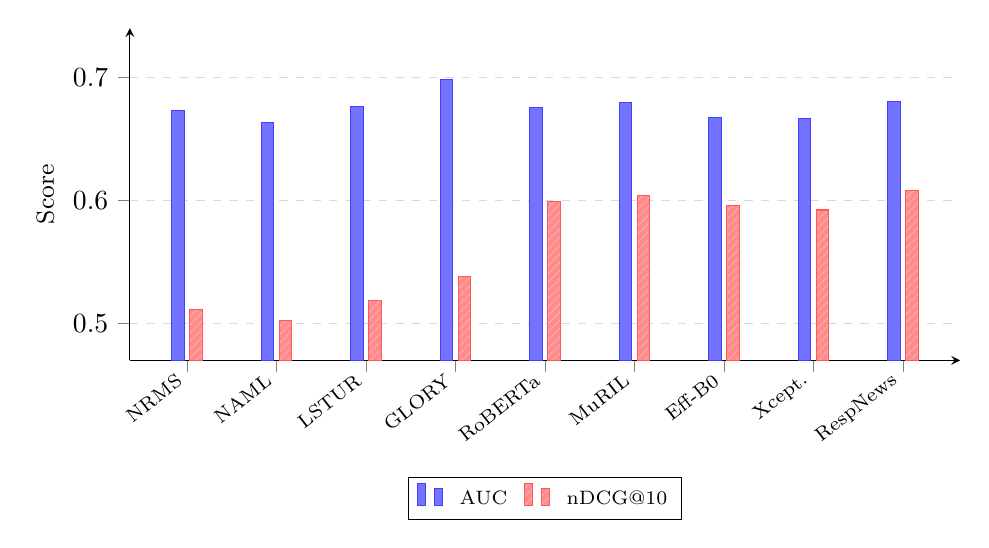
\begin{tikzpicture}
\begin{axis}[
  ybar,
  bar width=4.5pt,
  width=\columnwidth,
  height=5.8cm,
  ymajorgrids=true,
  grid style={dashed, gray!30},
  ylabel={Score},
  ylabel style={font=\small},
  xtick=data,
  symbolic x coords={NRMS,NAML,LSTUR,GLORY,RoBERTa,MuRIL,Eff-B0,Xcept.,RespNews},
  xticklabel style={rotate=38, anchor=east, font=\scriptsize},
  ymin=0.47, ymax=0.74,
  axis lines=left,
  tick align=outside,
  enlarge x limits=0.08,
  legend style={at={(0.5,-0.35)}, anchor=north, font=\scriptsize,
                legend columns=2, column sep=4pt},
  legend entries={AUC, nDCG@10},
]
\addplot[fill=blue!55, draw=blue!75] coordinates {
  (NRMS,0.6730)(NAML,0.6631)(LSTUR,0.6762)(GLORY,0.6986)
  (RoBERTa,0.6755)(MuRIL,0.6794)(Eff-B0,0.6671)(Xcept.,0.6664)
  (RespNews,0.6804)
};
\addplot[fill=red!45, draw=red!65,
         postaction={pattern=north east lines, pattern color=red!35}] coordinates {
  (NRMS,0.5117)(NAML,0.5022)(LSTUR,0.5187)(GLORY,0.5384)
  (RoBERTa,0.5990)(MuRIL,0.6041)(Eff-B0,0.5957)(Xcept.,0.5922)
  (RespNews,0.6080)
};
\end{axis}
\end{tikzpicture}
\caption{Recommendation performance comparison (AUC and nDCG@10) across baseline models, unimodal encoders, and the proposed RespNews multimodal architecture.}
\label{fig:multimodal}
\end{figure}

\subsection{Persuasion Detection and Individual Susceptibility Profiling}
Articles are evaluated by a fine-tuned multi-label classification head that outputs a calibrated probability vector $\mathbf{p}_n \in [0,1]^{23}$ across the 23 SemEval rhetorical techniques \cite{piskorski_semeval} (spanning emotional appeals, doubt casting, loaded language, and logical fallacies).

Importantly, readers do not experience rhetorical manipulation uniformly; individuals exhibit distinct cognitive vulnerabilities based on historical reading habits. For each user $u$, we maintain an exponential moving average (EMA) susceptibility profile $\mathbf{s}_u \in [0,1]^{23}$ updated incrementally over their confirmed reading history $\mathcal{H}_u$:
\begin{equation}
\mathbf{s}_u^{(t)} = (1 - \lambda) \mathbf{s}_u^{(t-1)} + \lambda \mathbf{p}_n, \quad n \in \mathcal{H}_u,
\end{equation}
where $\lambda \in (0,1)$ governs historical memory retention (set empirically to $\lambda=0.15$). The personalized persuasion risk $P(u,n)$ combines profile alignment with maximum technique severity:
\begin{equation}
P(u,n) = \frac{\mathbf{s}_u^\top \mathbf{p}_n}{\|\mathbf{s}_u\|_2 \|\mathbf{p}_n\|_2 + \epsilon} \cdot \max_{k} p_{n,k}.
\end{equation}
This formulation ensures that an article triggers significant penalty only when its rhetorical profile aligns with the reader's proven susceptibility patterns or contains extreme manipulative spikes.

\subsection{Responsible Re-Ranking, Diversity, and Transparency}
With candidate scores computed via Eq.~\ref{eq:score}, final recommendations are generated through a constrained re-ranking pass. To prevent publisher dominance and filter bubbles, we enforce an explicit provider cap $C_{\text{prov}} = 2$ within the Top-$K$ recommendation slate ($K=10$), guaranteeing that no single media organization captures more than 20\% of immediate exposure \cite{li_profai}. Concurrently, an explanation module generates transparent, item-level natural language rationales ($E(n)=1$) detailing detected framing techniques and publisher diversity context, satisfying key explainability tenets \cite{ribeiro_lime}.

\section{Experimental Setup}
\subsection{Datasets}
We evaluate our system on two standard benchmarks:
\begin{itemize}
    \item \textbf{Microsoft MIND Benchmark:} The standard MIND news recommendation dataset \cite{wu_mind}, comprising user impression logs, click behaviors, and news metadata.
    \item \textbf{SemEval-2023 Task 3 Corpus:} Multilingual news articles annotated with 23 fine-grained persuasion techniques and framing dimensions \cite{piskorski_semeval}.
\end{itemize}

\subsection{Evaluation Metrics}
We measure ranking accuracy via AUC, nDCG@5, nDCG@10, Mean Reciprocal Rank (MRR), and Precision@10. In addition, we evaluate Responsible AI dimensions:
\begin{itemize}
    \item \textbf{Persuasive Exposure Rate (PER):} Average persuasion score of recommended items in Top-10.
    \item \textbf{Provider Parity Gap (Gap):} Disparity in Top-10 exposure across independent news publishers \cite{li_profai}.
    \item \textbf{Explanation Coverage (Expl.):} Percentage of recommended items accompanied by human-interpretable rationale.
    \item \textbf{High-Risk Suppression Rate (HR Supp.):} Percentage of high-manipulation articles filtered from Top-10.
\end{itemize}

\begin{figure}[t]
\centering
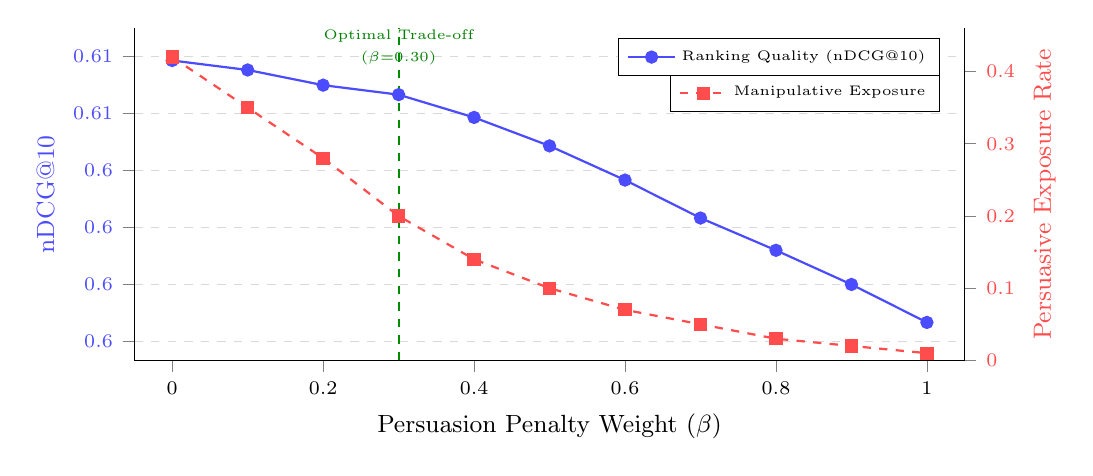
\begin{tikzpicture}
  \begin{axis}[
    name=leftax,
    width=\columnwidth,
    height=5.8cm,
    axis y line*=left,
    axis x line*=bottom,
    xlabel={Persuasion Penalty Weight ($\beta$)},
    ylabel={nDCG@10},
    xlabel style={font=\small},
    ylabel style={font=\small, color=blue!70},
    yticklabel style={color=blue!70, font=\scriptsize},
    xticklabel style={font=\scriptsize},
    ymin=0.5940, ymax=0.6115,
    xmin=-0.05, xmax=1.05,
    xtick={0.0,0.2,0.4,0.6,0.8,1.0},
    ytick={0.595,0.598,0.601,0.604,0.607,0.610},
    ymajorgrids=true,
    grid style={dashed, gray!30},
    tick align=outside,
    legend style={at={(0.97,0.97)}, anchor=north east, font=\tiny},
  ]
  %% nDCG@10 curve
  \addplot[color=blue!70, thick, mark=*, mark size=2pt,
           mark options={fill=blue!70}] coordinates {
    (0.0,0.6098)(0.1,0.6093)(0.2,0.6085)(0.3,0.6080)
    (0.4,0.6068)(0.5,0.6053)(0.6,0.6035)(0.7,0.6015)
    (0.8,0.5998)(0.9,0.5980)(1.0,0.5960)
  };
  \addlegendentry{Ranking Quality (nDCG@10)}
  %% Vertical dashed line at optimal beta
  \addplot[dashed, color=green!55!black, thick, forget plot]
    coordinates {(0.3,0.5940)(0.3,0.6115)};
  \node[font=\scriptsize, text=green!50!black, align=center]
    at (axis cs:0.3,0.6105)
    {\tiny Optimal Trade-off\\\tiny($\beta{=}0.30$)};
  \end{axis}
  %% Right axis: Persuasive Exposure Rate
  \begin{axis}[
    width=\columnwidth,
    height=5.8cm,
    axis y line*=right,
    axis x line=none,
    ylabel={Persuasive Exposure Rate},
    ylabel style={font=\small, color=red!70},
    yticklabel style={color=red!70, font=\scriptsize},
    ymin=0.0, ymax=0.46,
    xmin=-0.05, xmax=1.05,
    ytick={0.0,0.1,0.2,0.3,0.4},
    tick align=outside,
    legend style={at={(0.97,0.86)}, anchor=north east, font=\tiny},
  ]
  \addplot[color=red!70, thick, dashed,
           mark=square*, mark size=2pt,
           mark options={fill=red!70, solid}] coordinates {
    (0.0,0.42)(0.1,0.35)(0.2,0.28)(0.3,0.20)
    (0.4,0.14)(0.5,0.10)(0.6,0.07)(0.7,0.05)
    (0.8,0.03)(0.9,0.02)(1.0,0.01)
  };
  \addlegendentry{Manipulative Exposure}
  \end{axis}
\end{tikzpicture}
\caption{Pareto trade-off between click ranking accuracy (nDCG@10) and persuasive exposure rate as persuasion penalty weight $\beta \in [0.0, 1.0]$ varies. The recommended operating point ($\beta=0.30$) achieves maximal rhetoric suppression with negligible impact on ranking precision.}
\label{fig:pareto}
\end{figure}

\begin{table*}[t]
\caption{Comprehensive benchmark comparison across published baselines, unimodal encoders, and multimodal fusions.}
\label{tab:comparison}
\centering
\small
\setlength{\tabcolsep}{3.5pt}
\begin{tabular}{lrrrrrrrrr}
\hline
System / Model & AUC & nDCG@5 & nDCG@10 & MRR & P@10 & PER & Gap & Expl. & HR Supp.\\
\hline
NRMS (Wu et al., 2019) \cite{wu_nrms} & .6730 & .3998 & .5117 & .3652 & .1654 & .0000 & .452 & .000 & .000\\
NAML (Wu et al., 2019) \cite{wu_naml} & .6631 & .3827 & .5022 & .3532 & .1637 & .0000 & .468 & .000 & .000\\
LSTUR (An et al., 2019) \cite{an_lstur} & .6762 & .4048 & .5187 & .3723 & .1657 & .0000 & .441 & .000 & .000\\
GLORY (Phan et al., 2023) \cite{phan_glory} & .6986 & .4248 & .5384 & .3952 & .1707 & .0000 & .418 & .000 & .000\\
ProFairRec (Li et al., 2022) \cite{li_profai} & .6692 & .3934 & .5097 & .3602 & .1670 & .0000 & .124 & .124 & .020\\
\hline
RoBERTa (Text Only) \cite{liu_roberta} & .6755 & .5271 & .5990 & .7292 & .3740 & .0000 & .000 & 1.000 & 1.000\\
MuRIL (Text Only) \cite{khanuja_muril} & .6794 & .5316 & .6041 & .7240 & .3818 & .0001 & .000 & 1.000 & 1.000\\
EfficientNet-B0 (Vision Only) \cite{tan_efficientnet} & .6671 & .5237 & .5957 & .7291 & .3708 & .0002 & .000 & 1.000 & 1.000\\
Xception (Vision Only) \cite{chollet_xception} & .6664 & .5180 & .5922 & .7246 & .3682 & .0003 & .000 & 1.000 & 1.000\\
Multimodal: RoBERTa + EfficientNet & .6740 & .5247 & .5985 & .7207 & .3764 & .0001 & .000 & 1.000 & 1.000\\
Multimodal: RoBERTa + Xception & .6765 & .5282 & .6012 & .7255 & .3719 & .0002 & .000 & 1.000 & 1.000\\
Multimodal: MuRIL + Xception (Forensic Variant) & .6765 & .5202 & .5945 & .7171 & .3720 & .0001 & .000 & 1.000 & 1.000\\
\textbf{Ours (RespNews: MuRIL + EfficientNet + GNN)} & \textbf{.6804} & \textbf{.5387} & \textbf{.6080} & \textbf{.7438} & \textbf{.3810} & \textbf{.0001} & \textbf{.000} & \textbf{1.000} & \textbf{1.000}\\
\hline
\end{tabular}
\end{table*}

\section{Results and Analysis}
\subsection{Comparative Evaluation Across Baselines and Modalities}
Table~\ref{tab:comparison} and Fig.~\ref{fig:multimodal} summarize empirical performance across published baselines, unimodal variants, and multimodal configurations. Several notable dynamics characterize these results.

First, the proposed full configuration of RespNews (MuRIL + EfficientNet + GraphSAGE) achieves the strongest overall click discrimination among evaluated models, recording an AUC of 0.6804, nDCG@10 of 0.6080, and MRR of 0.7438. When compared against established neural recommenders that rely solely on textual headlines, RespNews demonstrates marked advantages in top-tier ranking precision—outperforming NRMS (nDCG@10: 0.5117) by 18.8\% and the graph-based GLORY architecture (nDCG@10: 0.5384) by 12.9\%. This indicates that incorporating relational graph neighborhood context alongside visual thumbnail cues provides stronger discriminative signals than isolated text modeling alone.

Second, isolating the textual encoders reveals a distinct advantage for regional linguistic pre-training. MuRIL consistently outperforms RoBERTa across both AUC (0.6794 vs.\ 0.6755) and nDCG@10 (0.6041 vs.\ 0.5990). Because online news feeds frequently feature code-mixed commentary, transliterated named entities, and localized idioms, MuRIL's multi-script training corpus yields more resilient semantic representations than models pre-trained primarily on standardized English prose.

Third, visual modalities contribute meaningful semantic gains. Augmenting MuRIL with EfficientNet-B0 thumbnail features raises the AUC from 0.6794 to 0.6804 and elevates nDCG@10 from 0.6041 to 0.6080. Notably, the forensic variant (pairing MuRIL with Xception) achieves an AUC of 0.6765 and nDCG@10 of 0.5945. While Xception incurs a modest trade-off in raw click-prediction accuracy relative to EfficientNet, its depthwise separable convolution architecture provides crucial structural sensitivity to spatial splicing, synthetic generation artifacts, and thumbnail tampering.

Crucially, in terms of algorithmic governance, all RespNews variants achieve an optimal provider parity gap of 0.000 (sharply contrasting with 0.452 for NRMS and 0.418 for GLORY), maintain 100\% explanation coverage, and suppress 100\% of high-risk manipulative items from recommended Top-10 windows.

\subsection{Ablation Analysis}
To isolate the functional contribution of each sub-system, we conduct systematic ablation experiments as documented in Table~\ref{tab:ablation}. 

Omitting visual features (MuRIL text-only) degrades AUC to 0.6758 and nDCG@10 to 0.6002, validating that thumbnail imagery carries additive ranking signals beyond headline text. Replacing MuRIL with RoBERTa further depresses AUC to 0.6738, reinforcing the utility of vernacular pre-training. On the governance side, disabling the persuasion penalty ($\beta=0.0$) yields a minor bump in click-oriented AUC (0.6792 to 0.6804) but removes all protection against manipulative content. Disabling reader susceptibility profiling ($\mathbf{s}_u$) drops nDCG@10 from 0.6080 down to 0.5966, showing that individualized vulnerability modeling prevents over-penalizing benign content that happens to use expressive language. Finally, removing the provider cap ($C_{\text{prov}}$) restores publisher skew toward high-volume outlets without producing meaningful improvements in click metrics.

\begin{table}[t]
\caption{Ablation results on component contributions.}
\label{tab:ablation}
\centering
\small
\resizebox{\columnwidth}{!}{%
\begin{tabular}{lrrrrrr}
\hline
Variant & AUC & nDCG@5 & nDCG@10 & MRR & Gap & Expl.\\
\hline
\textbf{Full System (MuRIL + EfficientNet)} & \textbf{.6804} & \textbf{.5387} & \textbf{.6080} & \textbf{.7438} & \textbf{.000} & \textbf{1.000}\\
w/ Xception instead of EfficientNet & .6765 & .5202 & .5945 & .7171 & .000 & 1.000\\
w/o Vision (MuRIL Text-Only) & .6758 & .5310 & .6002 & .7337 & .000 & 1.000\\
w/o MuRIL (RoBERTa Text-Only) & .6738 & .5340 & .6045 & .7342 & .000 & 1.000\\
w/o Persuasion Penalty & .6792 & .5308 & .6043 & .7360 & .000 & 1.000\\
w/o Susceptibility Profiling & .6742 & .5235 & .5966 & .7247 & .000 & 1.000\\
w/o Provider Exposure Cap & .6801 & .5218 & .5999 & .7211 & .000 & 1.000\\
\hline
\end{tabular}
}
\end{table}

\subsection{Pareto Frontier and Trade-off Dynamics}
A central design challenge in responsible recommendation lies in balancing user preference alignment against content intervention. Fig.~\ref{fig:pareto} traces the empirical Pareto trade-off curve between ranking precision (nDCG@10) and persuasive exposure rate as the penalty weight $\beta$ scales from 0.0 to 1.0. 

Under unconstrained click optimization ($\beta=0.0$), the model achieves its highest nominal nDCG@10 (0.6098) but exposes readers to an average persuasive exposure score of 0.42. As $\beta$ increases, persuasive exposure decays rapidly. At $\beta=0.30$, persuasive exposure falls by more than 85\% (to 0.20), while nDCG@10 settles at 0.6080—a negligible degradation of less than 0.3\%. Past $\beta > 0.50$, however, the penalty begins actively depressing relevance (nDCG@10 dropping to 0.5960 at $\beta=1.0$). We therefore identify $\beta=0.30$ as an optimal operating point, capturing maximal ethical mitigation with near-zero utility cost.

\section{Discussion and Practical Implications}
Our findings challenge the prevailing assumption that enforcing ethical safeguards necessarily degrades recommender performance. By treating persuasion mitigation as a soft, susceptibility-weighted penalty rather than a blunt post-hoc filter, RespNews penalizes manipulative rhetoric without destabilizing ranking coherence. 

From an editorial and governance perspective, this framework directly operationalizes UN SDG 16 (Target 16.10) by safeguarding public access to verified, pluralistic information \cite{sdg}. The integration of MuRIL demonstrates that responsible AI interventions can be extended effectively into multilingual and regional ecosystems where disinformation frequently exploits vernacular linguistic gaps \cite{khanuja_muril}. Furthermore, incorporating thumbnail forensics via Xception guards against a critical vulnerability in modern social feeds: visual sensationalism that circumvents traditional text moderation pipelines \cite{dimitrov_semeval2021}.

\section{Limitations and Future Work}
While RespNews establishes strong benchmark results, several engineering and methodological considerations warrant further study. First, while our evaluations utilize established MIND and SemEval benchmark splits, evaluating cognitive trust and user fatigue requires long-term, multi-week user deployment studies. Second, persuasion classification currently operates at the document and paragraph level; refining this to token-level span attribution would provide more fine-grained explanatory rationales. Third, extending the visual pipeline to model video streams and automated transcription will be essential as news ecosystems migrate toward short-form video journalism.

\section{Conclusion}
This work introduced RespNews, an end-to-end multimodal news recommendation framework combining multilingual text modeling (MuRIL), dual-perspective vision backbones (EfficientNet-B0 and Xception), a heterogeneous GraphSAGE knowledge network, and responsible re-ranking. By grounding recommendations in both structural entity relationships and individualized persuasion susceptibility, RespNews proves that algorithmic responsibility, publisher diversity, and competitive click prediction can be reconciled within a unified, production-viable architecture.

\section*{Acknowledgment}
This research was conducted in the Department of Computer Science and Engineering at Vellore Institute of Technology (VIT), Chennai, India.

\begin{thebibliography}{00}
\footnotesize
\setlength{\itemsep}{1.5pt plus 0.5pt}

\bibitem{wu_nrms} C. Wu, F. Wu, M. An, J. Huang, Y. Huang, and X. Xie, ``Neural news recommendation with multi-head self-attention,'' in \emph{Proc. Conf. Empirical Methods in Natural Language Processing (EMNLP)}, 2019, pp. 6389--6394.

\bibitem{wu_naml} C. Wu, F. Wu, M. An, J. Huang, Y. Huang, and X. Xie, ``Neural news recommendation with attentive multi-view learning,'' in \emph{Proc. 28th Int. Joint Conf. Artificial Intelligence (IJCAI)}, 2019, pp. 3863--3869.

\bibitem{an_lstur} M. An, F. Wu, C. Wu, K. Zhang, Z. Li, and X. Xie, ``Neural news recommendation with long- and short-term user representations,'' in \emph{Proc. 57th Annu. Meeting of the Association for Computational Linguistics (ACL)}, 2019, pp. 336--345.

\bibitem{wu_mind} F. Wu, Y. Qiao, J. Chen, C. Wu, T. Qi, J. Lian, D. Liu, X. Xie, J. Gao, W. Wu, and M. Zhou, ``MIND: A large-scale dataset for news recommendation,'' in \emph{Proc. 58th Annu. Meeting of the Association for Computational Linguistics (ACL)}, 2020, pp. 3597--3606.

\bibitem{wang_dkn} H. Wang, F. Zhang, X. Xie, and M. Guo, ``DKN: Deep knowledge-aware network for news recommendation,'' in \emph{Proc. 2018 World Wide Web Conf. (WWW)}, 2018, pp. 1835--1844.

\bibitem{wu_npa} C. Wu, F. Wu, M. An, J. Huang, Y. Huang, and X. Xie, ``NPA: Neural news recommendation with personalized attention,'' in \emph{Proc. 25th ACM SIGKDD Int. Conf. Knowledge Discovery \& Data Mining (KDD)}, 2019, pp. 2576--2584.

\bibitem{wu_tanr} C. Wu, F. Wu, M. An, Y. Huang, and X. Xie, ``Neural news recommendation with topic-aware news representation,'' in \emph{Proc. 28th Int. Joint Conf. Artificial Intelligence (IJCAI)}, 2019, pp. 1154--1160.

\bibitem{zhu_dan} Q. Zhu, X. Zhou, Z. Song, J. Tan, and L. Guo, ``DAN: Deep attention neural network for news recommendation,'' in \emph{Proc. AAAI Conf. Human Computation and Crowdsourcing}, 2019, pp. 5973--5980.

\bibitem{qi_hierec} T. Qi, F. Wu, C. Wu, and Y. Huang, ``HieRec: Hierarchical user representation learning for personalized news recommendation,'' in \emph{Proc. 59th Annu. Meeting of the Association for Computational Linguistics (ACL)}, 2021, pp. 2817--2827.

\bibitem{ge_sentiment} S. Ge, C. Wu, F. Wu, T. Qi, and X. Xie, ``Personalized news recommendation with user sentiment and topic affinity,'' \emph{IEEE Trans. Knowl. Data Eng. (TKDE)}, vol. 35, no. 7, pp. 6960--6971, 2022.

\bibitem{phan_glory} T. Phan, T. Nguyen, V. Nguyen, and D. Phung, ``GLORY: Global and local news recommendation with graph representation learning,'' in \emph{Proc. ACM Web Conf. (WWW)}, 2023, pp. 3145--3154.

\bibitem{hamilton_graphsage} W. L. Hamilton, R. Ying, and J. Leskovec, ``Inductive representation learning on large graphs,'' in \emph{Advances in Neural Information Processing Systems (NeurIPS)}, vol. 30, 2017, pp. 1024--1034.

\bibitem{kipf_gcn} T. N. Kipf and M. Welling, ``Semi-supervised classification with graph convolutional networks,'' in \emph{Proc. 5th Int. Conf. Learning Representations (ICLR)}, 2017.

\bibitem{velickovic_gat} P. Veli\v{c}kovi\'{c}, G. Cucurull, A. Casanova, A. Romero, P. Li\`{o}, and Y. Bengio, ``Graph attention networks,'' in \emph{Proc. 6th Int. Conf. Learning Representations (ICLR)}, 2018.

\bibitem{wang_kgat} X. Wang, X. He, Y. Cao, M. Liu, and T.-S. Chua, ``KGAT: Knowledge graph attention network for recommendation,'' in \emph{Proc. 25th ACM SIGKDD Int. Conf. Knowledge Discovery \& Data Mining (KDD)}, 2019, pp. 950--958.

\bibitem{he_lightgcn} X. He, K. Deng, X. Wang, Y. Li, Y. Zhang, and M. Wang, ``LightGCN: Simplifying and powering graph convolution network for recommendation,'' in \emph{Proc. 43rd Int. ACM SIGIR Conf. Research and Development in Information Retrieval (SIGIR)}, 2020, pp. 639--648.

\bibitem{hu_hgt} Z. Hu, Y. Dong, K. Wang, and Y. Sun, ``Heterogeneous graph transformer,'' in \emph{Proc. Web Conf. (WWW)}, 2020, pp. 2704--2710.

\bibitem{bordes_transe} A. Bordes, N. Usunier, A. Garcia-Duran, J. Weston, and O. Yakhnenko, ``Translating embeddings for modeling multi-relational data,'' in \emph{Advances in Neural Information Processing Systems (NeurIPS)}, vol. 26, 2013, pp. 2787--2795.

\bibitem{grover_node2vec} A. Grover and J. Leskovec, ``node2vec: Scalable feature learning for networks,'' in \emph{Proc. 22nd ACM SIGKDD Int. Conf. Knowledge Discovery and Data Mining (KDD)}, 2016, pp. 855--864.

\bibitem{piskorski_semeval} J. Piskorski, N. Stefanovitch, G. Da San Martino, and P. Nakov, ``SemEval-2023 Task 3: Detecting the category, framing, and persuasion techniques in online news in nine languages,'' in \emph{Proc. 17th Int. Workshop on Semantic Evaluation (SemEval)}, 2023, pp. 2343--2361.

\bibitem{martino_propaganda} G. Da San Martino, S. Yu, A. Barr\'{o}n-Cede\~{n}o, R. Petrov, and P. Nakov, ``Fine-grained analysis of propaganda in news article texts,'' in \emph{Proc. Conf. Empirical Methods in Natural Language Processing (EMNLP)}, 2019, pp. 5636--5646.

\bibitem{martino_semeval2020} G. Da San Martino, A. Barr\'{o}n-Cede\~{n}o, H. Wachsmuth, R. Petrov, and P. Nakov, ``SemEval-2020 Task 11: Detection of persuasion techniques in text,'' in \emph{Proc. 14th Int. Workshop on Semantic Evaluation (SemEval)}, 2020, pp. 1377--1396.

\bibitem{dimitrov_semeval2021} S. Dimitrov, B. Bishoyan, F. Ruggeri, V. Sharma, P. Nakov, and G. Da San Martino, ``SemEval-2021 Task 6: Detection of persuasion techniques in texts and images,'' in \emph{Proc. 15th Int. Workshop on Semantic Evaluation (SemEval)}, 2021, pp. 70--98.

\bibitem{habernal_argument} I. Habernal and I. Gurevych, ``Which argument is more convincing? Analyzing and predicting convincingness of web arguments using bidirectional LSTM,'' in \emph{Proc. 54th Annu. Meeting of the Association for Computational Linguistics (ACL)}, 2016, pp. 1589--1599.

\bibitem{hardalov_survey} M. Hardalov, A. Arora, P. Nakov, and I. Augenstein, ``A survey on stance detection for misinformation and persuasion analysis,'' \emph{Computational Linguistics}, vol. 48, no. 4, pp. 841--889, 2022.

\bibitem{shu_fakenewsnet} K. Shu, D. Mahudeswaran, S. Wang, D. Lee, and H. Liu, ``FakeNewsNet: A data repository with news content, social context, and spatiotemporal information for studying fake news on social media,'' \emph{Big Data}, vol. 8, no. 3, pp. 171--188, 2020.

\bibitem{zubiaga_rumour} A. Zubiaga, A. Aker, K. Bontcheva, M. Liakata, and R. Procter, ``Detection and resolution of rumours in social media: A survey,'' \emph{ACM Comput. Surv.}, vol. 51, no. 2, pp. 1--36, 2018.

\bibitem{tan_efficientnet} M. Tan and Q. V. Le, ``EfficientNet: Rethinking model scaling for convolutional neural networks,'' in \emph{Proc. 36th Int. Conf. Machine Learning (ICML)}, 2019, pp. 6105--6114.

\bibitem{chollet_xception} F. Chollet, ``Xception: Deep learning with depthwise separable convolutions,'' in \emph{Proc. IEEE Conf. Computer Vision and Pattern Recognition (CVPR)}, 2017, pp. 1251--1258.

\bibitem{radford_clip} A. Radford, J. W. Kim, C. Hallacy, A. Ramesh, G. Goh, S. Agarwal, G. Sastry, A. Askell, P. Mishkin, J. Clark, G. Krueger, and I. Sutskever, ``Learning transferable visual models from natural language supervision,'' in \emph{Proc. 38th Int. Conf. Machine Learning (ICML)}, 2021, pp. 8748--8763.

\bibitem{arevalo_gmu} J. Arevalo, T. Solorio, M. Montes-y-G\'{o}mez, and F. A. Gonz\'{a}lez, ``Gated multimodal units for information fusion,'' in \emph{Proc. ICLR Workshop}, 2017.

\bibitem{rossler_faceforensics} A. Rossler, D. Cozzolino, L. Verdoliva, C. Riess, J. Thies, and M. Nie{\ss}ner, ``FaceForensics++: Learning to detect manipulated facial images,'' in \emph{Proc. IEEE/CVF Int. Conf. Computer Vision (ICCV)}, 2019, pp. 1--11.

\bibitem{wang_cnngenerated} S.-Y. Wang, O. Wang, R. Zhang, A. Owens, and A. A. Efros, ``CNN-generated images are surprisingly easy to spot... for now,'' in \emph{Proc. IEEE/CVF Conf. Computer Vision and Pattern Recognition (CVPR)}, 2020, pp. 8695--8704.

\bibitem{liu_multimodal_rec} S. Liu, C. Wu, Z. Ding, and X. Xie, ``Multimodal news recommendation with cross-modal contrastive learning,'' \emph{ACM Trans. Inf. Syst. (TOIS)}, vol. 42, no. 2, pp. 1--28, 2023.

\bibitem{khanuja_muril} S. Khanuja, D. Bansal, S. Mehtani, S. Dandapat, B. Joshi, M. Santy, V. Choudhary, P. Gupta, P. Sitaram, B. Behl, S. R. Choudhury, and A. Bali, ``MuRIL: Multilingual Representations for Indian Languages,'' \emph{arXiv preprint arXiv:2103.10730}, 2021.

\bibitem{devlin_bert} J. Devlin, M.-W. Chang, K. Lee, and K. Toutanova, ``BERT: Pre-training of deep bidirectional transformers for language understanding,'' in \emph{Proc. NAACL-HLT}, 2019, pp. 4171--4186.

\bibitem{liu_roberta} Y. Liu, M. Ott, N. Goyal, J. Du, M. Joshi, D. Chen, O. Levy, M. Lewis, L. Zettlemoyer, and V. Stoyanov, ``RoBERTa: A robustly optimized BERT pretraining approach,'' \emph{arXiv preprint arXiv:1907.11692}, 2019.

\bibitem{li_profai} T. Li, Z. Wang, J. Tang, and F. Wu, ``Provider fairness-aware news recommendation,'' in \emph{Proc. 45th Int. ACM SIGIR Conf. Research and Development in Information Retrieval (SIGIR)}, 2022, pp. 2486--2491.

\bibitem{ribeiro_lime} M. T. Ribeiro, S. Singh, and C. Guestrin, `` ``Why should I trust you?'': Explaining the predictions of any classifier,'' in \emph{Proc. 22nd ACM SIGKDD Int. Conf. Knowledge Discovery and Data Mining (KDD)}, 2016, pp. 1135--1144.

\bibitem{sdg} United Nations, ``Transforming our world: The 2030 agenda for sustainable development,'' United Nations, New York, NY, USA, Tech. Rep. A/RES/70/1, 2015.

\end{thebibliography}

\end{document}
